\documentclass{article}

\usepackage{amsmath}
\usepackage[utf8]{inputenc}
\usepackage{amssymb}
\usepackage{geometry}
\usepackage{fancyhdr}
\usepackage{tikz}
\usepackage{mdframed}
\usepackage{xcolor}
\usepackage[unicode=true, colorlinks=true, linkcolor=black, urlcolor=blue, citecolor=blue]{hyperref}

\definecolor{lightorange}{HTML}{f7d6e0}
% Define the question environment
\newenvironment{question}
{\begin{mdframed}[backgroundcolor=white]}
{\end{mdframed}}

% Define the solution environment
\newenvironment{solution}
{\begin{mdframed}[backgroundcolor=lightorange,hidealllines=true]}
{\end{mdframed}}

% Page setup
\geometry{a4paper, margin=2cm}
\pagestyle{fancy}
\fancyhf{}
\lhead{I2 Review}
\rhead{\today}

\begin{document}

\begin{titlepage}
    \centering
    \vspace*{2cm}
    {\Huge\bfseries Optimizacion - EX}\\[1cm]
    \vspace{1cm}
    {\Large Nombre: \par}
    {\large Sebastian Lorca\par}
    \vspace{0.5cm}
    {\Large Date: \par}
    {\large \today \par}
    \vspace{0.5cm}
    {\Large Profesor: \par}
    {\large Raimundo Cuadrado\par}
    \vspace{0.5cm}
    {\Large Email: \par}
    {\large \href{mailto:sdlorca@uc.cl}{sdlorca@uc.cl}\par}
    \vspace{0.5cm}
    {\Large Sigla: \par}
    {\large ICS1113\par}
    \vspace{0.5cm}
    {\Large Semestre: \par}
    {\large 1/2024\par}
    \vspace{1cm}
\end{titlepage}
\tableofcontents
\newpage


\section{Programaci\'on Entera}

Un problema general de programación entera es:

\begin{align*}
    \min \quad & c^T x \\
    \text{s.a.} \quad & Ax = b \\
    & x \geq 0 \\
    & x \in \mathbb{Z}^n
\end{align*}

\subsection{Relajación Lineal}

La relajación lineal de un problema de programación entera es:

\begin{align*}
    \min \quad & z^* = c^T x & \sim && z^o = c^T x \\
    \text{s.a.} \quad & Ax = b & && Ax = b \\
    & x \geq 0 &&& x \geq 0 \\
    & x \in \mathbb{Z}^n &&& x \in \mathbb{R}^n
\end{align*}

Como el problema se relaja, se tiene que $z^o \leq z^*$, ya que el problema relajado tiene un dominio factible mayor.

\subsection{Branch and Bound}

Asumiendo un problema de programación entera $S$ acotado, se puede ocupar la técnica de relajación lineal y obtener:

\begin{align*}
    \text{P}_0) \quad & z^o = c^T x \\
    & Ax = b \\
    & x \geq 0 \\
    & x \in \mathbb{R}^n
\end{align*}

Y ocupando Simplex resolver el problema relajado, es decir, $z_o = c^T x_o$. Si $x_o$ tiene alguna entrada fraccionaria, se puede ocupar la técnica de \textbf{Branch and Bound}.

\subsubsection{Branch}

Si $x_o$ tiene alguna entrada fraccionaria, se puede seleccionar una variable $x_j$ con valor fraccionario y se puede crear dos subproblemas:

\begin{align*}
    \text{P}_1) \quad & z^o = c^T x \\
    & Ax = b \\
    & x \geq 0 \\
    & x \in \mathbb{R}^n \\
    & x_j \leq \lfloor x_j \rfloor
\end{align*}

\begin{align*}
    \text{P}_2) \quad & z^o = c^T x \\
    & Ax = b \\
    & x \geq 0 \\
    & x \in \mathbb{R}^n \\
    & x_j \geq \lceil x_j \rceil
\end{align*}

\subsubsection{Bound}

Si $x_o$ no tiene ninguna entrada fraccionaria, se puede comparar $z^o$ con el mejor valor entero encontrado hasta el momento, el \textit{incumbente}. Si $z^o$ es mejor, se actualiza el mejor valor entero encontrado.

Repitiendo el proceso de Branch and Bound, se puede encontrar la solución óptima del problema de programación entera generando un árbol de soluciones:

\begin{center}
    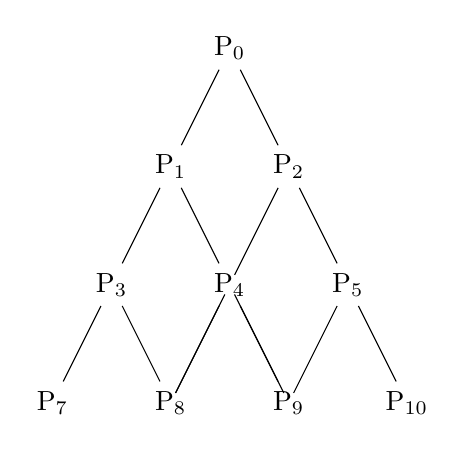
\begin{tikzpicture}
        \node {P$_0$}
            child {node {P$_1$}
                child {node {P$_3$}
                    child {node {P$_7$}}
                    child {node {P$_8$}}
                }
                child {node {P$_4$}
                    child {node {}}
                    child {node {P$_{9}$}}
                }
            }
            child {node {P$_2$}
                child {node {}
                    child {node {}}
                    child {node {}}
                }
                child {node {P$_5$}
                    child {node {}}
                    child {node {P$_{10}$}}
                }
            };
    \end{tikzpicture}
\end{center}

\subsection{Branch and Cut}

La técnica de \textbf{Branch and Cut} es una extensión de \textbf{Branch and Bound} que incluye cortes para acelerar la convergencia del algoritmo.

\subsubsection{Cortes de Gomory}

\begin{enumerate}
    \item Se expresan los coeficientes de cada restricción como la suma de un entero y una fracción no negativa.
    \item Se eliminan los términos enteros y se cambia $=$ por $\geq$.
\end{enumerate}

\textbf{Ejemplo:}

\begin{flalign*}
    &&0x_1-\frac{3}{4}x_2+\frac{1}{3}x_3-3\frac{1}{4}x_4 &= 10\frac{3}{7}& \\
    &\text{Paso 1:}\\
    &&(-1 + \frac{1}{4})x_2 + (0 + \frac{1}{3})x_3 + (-4  + \frac{3}{4})x_4 &= 10 +\frac{3}{7}& \\
    &\text{Paso 2:}\\
    &&\frac{1}{4}x_2 + \frac{1}{3}x_3 + \frac{3}{4}x_4 &\geq \frac{3}{7}& \\
\end{flalign*}

Más información \href{https://www.ou.edu/class/che-design/che5480-11/Gomory%20Cuts-The%20How%20and%20the%20Why.pdf}{acá}

\subsubsection{Cortes de Cover}

Para restricciones que son la suma de variables binarias con coeficientes no negativos que sea menor o igual a un valor no negativo, entonces es posible agregar un corte de Cover.

Se expresa de la forma:

\begin{align*}
    \sum_{j \in J} a_j x_j \leq b\\
    \text{Donde } a_j \geq 0 \text{ y } b \geq 0
    x \in \{0, 1\}^n
\end{align*}

Y el corte de Cover se expresa como:

\begin{align*}
    \sum_{j \in J} x_j \leq |J| - 1
\end{align*}

Información de MIP \href{https://optimization.cbe.cornell.edu/index.php?title=Mixed-integer_cuts}{acá}.

\section{Programaci\'on No Lineal}

\subsection{Optimizaci\'on sin restricciones}

Para clasificar funciones, se denominaran de clase $C^k$ si todas sus derivadas parciales de orden $k$ son continuas \footnote{Una fución derivable es continua, pero una función continua no necesariamente es derivable.}.

\subsubsection{Condiciones necesarias de primer orden}

\textbf{Teorema de Fermat:} (Sea $f(x)$ continuamente derivable) Si $f(x)$ tiene un máximo o mínimo local en $x_0$, y $f(x)$ es derivable en $x_0$, entonces $f'(x_0) = 0$.

\textbf{Teorema de Fermat generalizado:} (Sea $f(x)$ continuamente derivable) Si $f(x)$ tiene un máximo o mínimo local en $x_0$, y $f(x)$ es derivable en $x_0$, entonces $\nabla f(x_0) = 0$.

\subsubsection{Condicion necesaria de segundo orden}

Si $x^*$ es mínimo local de $f$, entonces $\nabla^2f(x^*)$ es semidefinida positiva. Esto es llamado el \textbf{Criterio de la Segunda Derivada}.

\subsubsection{Condición Suficiente de Segundo Orden}

Si $f:D\to R$ de clase $C^2$. Sea $x^* \in D$ con $\nabla f(x^*)=0$ (punto crítico):

\begin{enumerate}
    \item Si $\nabla^2f(x^*)=H(f(x^*)) > 0$ entonces $x^*$ es un mínimo local \textit{estricto} de $f$.
    \item Si $\nabla^2f(x^*)=H(f(x^*)) < 0$ entonces $x^*$ es un máximo local \textit{estricto} de $f$.
    \item Si $\nabla^2f(x^*)=H(f(x^*))$ es indefinida, entonces $x^*$ es un punto silla.
\end{enumerate}

Si $f$ es convexa, cualquier mínimo local $x^*$ es mínimo global de $f$. Si esta es diferenciable, entonces cualquier punto crítico $x^*$ es mínimo global de $f$.

\subsubsection{Relación con Convexidad}

\textbf{Teorema:} Sea $f:D \subseteq \mathbb{R}^n \to \mathbb{R}$ dos veces continuamente diferenciable, con $D$ convexo. Entonces:

\begin{enumerate}
    \item $f$ es convexa si y solo si $\nabla^2 f(x)$ es semidefinida positiva para todo $x \in D$.
    \item Si $\nabla^2 f(x)$ es definida positiva para todo $x \in D$, entonces $f$ es estrictamente convexa.
\end{enumerate}

\subsubsection{Método del Gradiente (o de Cauchy)}

El método del gradiente es un método iterativo para encontrar un mínimo local de una función. Se dice que "la función decrece en la dirección del negativo del gradiente". Así:

\begin{equation*}
    f(x+\lambda d) < f(x) \quad \forall \lambda \in (0, r]
\end{equation*}

Donde $d$ es la dirección de descenso. Si $d^T \nabla f(x) < 0$, entonces $d$ es una dirección de descenso.

\textbf{Algoritmo:}

\begin{enumerate}
    \item Sea $x^0 \in \mathbb{R}^n$ un punto inicial, $k=0$.
    \item Sea $d^k = -\nabla f(x^k)$ la dirección de descenso.
    \item Si $||\nabla f(x^k)|| < \varepsilon$, entonces $x^k$ es un mínimo local.
    \item Sino, resolver aproximadamente $\min_{\lambda>0} f(x^k + \lambda d^k)$.
    \item Sea $x^{k+1}=x^k + \lambda d^k$. $k = k+1$ (volver al paso 2).
\end{enumerate}

Bajo condiciones razonables el modelo converge a un punto estacionario (punto crítico) de $f$ (o a un punto cercano con el criterio de término). En caso que la función objetivo sea convexa, el método converge a un mínimo global. \textbf{Beneficio:} Es un método simple.

Si $x^*$ es un mínimo local, entonces existe $r>0$ tal que si el punto inicial $x^o$ cumple $||x^o - x^*|| < r$, entonces el método converge a $x^*$. A esto se le llama \textbf{Convergencia Local}.

\subsection{Optimizaci\'on con restricciones}

\subsubsection{Condiciones de Lagrange}

El \textbf{Teorema de Lagrange} para un problema:

\begin{align*}
    \text{minimizar} \quad & f(x) \\
    \text{sujeto a} \quad & g_i(x) = a_i \quad \forall i = 1, \ldots, m
\end{align*}

Se puede escribir como:

\begin{align*}
    \mathrm{L}(x, \lambda) = f(x) + \sum_{i=1}^r \lambda_i (g_i(x) - a_i)
\end{align*}

Donde $\lambda_i$ son los \textbf{Multiplicadores de Lagrange}, que se entienden como aquellos que miden la sensibilidad del valor óptimo de la función objetivo al cambio de los recursos $b_i$ de las restricciones en el problema. Estos multiplicadores, para un problema de $m$ restricciones, se expresan como $L(x_1, x_2, \dots, x_n, \lambda_1, \lambda_2, \dots, \lambda_n) - \sum_{i=1}^{m} \lambda_i g_i(x_1,x_2,\dots,x_n)$.

La solución óptima para los multiplicadores de lagrange se determina con las derivadas parciales de cada $x_n$ y $\lambda_i$ e igualando a cero. Así, se obtiene un sistema de ecuaciones que se resuelve para encontrar los valores óptimos de $x_n$ y $\lambda_i$.

Para encontrar los puntos críticos de $\mathrm{L}(x, \lambda)$, se deben resolver las siguientes ecuaciones:

\begin{align*}
    \nabla f(x) + \sum_{i=1}^r \lambda_i \nabla g_i(x) &= 0 \\
    g_i(x) &= a_i \quad \forall i = 1, \ldots, m
\end{align*}

Si $x^*$ es un mínimo local\dots


Primero se deben evaluar las condiciones de regularidad. Para esto, se debe evaluar la matriz jacobiana de $g(x)$ en $x^*$, y si esta matriz es de rango completo, entonces se cumple la condición de regularidad.

\begin{align*}
    \nabla f(x^*) + \sum_{i=1}^r \lambda_i \nabla g_i(x^*) &= 0 \\
    g_i(x^*) &= a_i \quad \forall i = 1, \ldots, m
\end{align*}

Luego, se debe evaluar la matriz hessiana de $\mathrm{L}(x, \lambda)$ en $(x^*, \lambda^*)$, y si esta matriz es definida positiva, entonces $x^*$ es un mínimo local.

Revisar \ref{problemas:lagrangiano}

\subsubsection{Condiciones de Karush-Kuhn-Tucker}

Sea $x \, \in \, D$. Denotemos por $I(x)={i:g_i(x)=b_i}$ el conjunto de índices de las restricciones activas en el punto $x$.

\textbf{Teorema de Karush-Kuhn-Tucker:}

Un conjunto $K \subset \mathbb{R}^n$ es convexo si y solo si para todo $x_1, x_2 \in K$ y $\lambda \in [0, 1]$, se tiene que $\lambda x_1 + (1 - \lambda) x_2 \in K$.

(Sea $f(x)$ y $g(x)$ continuamente derivables) Si $x_0$ es un mínimo local de $f(x)$ sujeto a $g(x) = 0$, entonces existen $\lambda_0, \lambda_1, \ldots, \lambda_m$ tales que:

\begin{align*}
    \nabla f(x_0) + \sum_{i=1}^{m} \lambda_i \nabla g_i(x_0) &= 0 \\
    \lambda_i g_i(x_0) &= 0 \quad \forall i = 1, \ldots, m \\
    \lambda_i &\geq 0 \quad \forall i = 1, \ldots, m
\end{align*}


\section{Problemas}

\subsection{Lagrange} \label{problemas:lagrangiano}

\begin{question}
    Extrahído de \href{https://www.bbau.ac.in/dept/UIET/EME-601%20Operation%20Research.pdf}{libro de problemas de optimización}.

    \begin{align*}
        z \quad&=f(x_1,x_2)=2x_1x_2\\
        \text{s.a.} \quad& x_1^2+x_2^2=1
    \end{align*}
\end{question}

\begin{solution}
    \begin{align*}
        L(x_1,x_2,\lambda) &= f(x_1,x_2) + \lambda(g(x_1,x_2)-1)\\
        &= 2x_1x_2 + \lambda(x_1^2+x_2^2-1)
    \end{align*}

    \begin{align*}
        \frac{\partial L}{\partial x_1} &= 2x_2 + 2\lambda x_1 = 0\\
        \frac{\partial L}{\partial x_2} &= 2x_1 + 2\lambda x_2 = 0\\
        \frac{\partial L}{\partial \lambda} &= x_1^2 + x_2^2 - 1 = 0
    \end{align*}

    Resolviendo el sistema de ecuaciones, se obtiene que $x_1 = \pm \frac{1}{\sqrt{2}}$ y $x_2 = \pm \frac{1}{\sqrt{2}}$.
\end{solution}

\subsection{KKT} \label{problemas:kkt}
\begin{question}
    Demuestre que para $f$ diferenciable y $x^*$ mínimo local, entonces $\nabla f(x^*)=0$.
\end{question}

\begin{solution}
    Asumiendo que $\nabla f(x^*)\neq 0$, entonces:
    \begin{align*}
        h&=-\nabla f(x^*)\\
        g(t)&=f(x^* + th) \quad \frac{\mathrm{g}}{\mathrm{d}t}\\
        g'(0)&=\nabla f(x^*)^T h\\
        g'(0)&=\nabla f(x^*)^T (-\nabla f(x^*))= -||\nabla f(x^*)||^2 < 0\\
        &\therefore g'(0) < 0
    \end{align*}
    Como $x^*$ es mínimo local, no puede haber un valor más pequeño, luego $\Rightarrow \! \Leftarrow$. Por lo tanto: $\nabla f(x^*)=0$.
\end{solution}

\begin{question}
    Al resolver un problema de Programación lineal hasta el óptimo se obtiene una solución en donde una variable no básica tiene costo reducido nulo. ¿Significa necesariamente esto que existe otro punto extremo del problema que también es solución optima?
\end{question}

\begin{solution}
    No, no necesariamente. Si bien es cierto que si una variable no básica tiene costo reducido nulo, entonces el problema tiene soluciones múltiples, no necesariamente todas las soluciones múltiples son óptimas.
\end{solution}

\begin{question}
    \begin{align*}
        \min \quad & x^2+y^2 \\
        \text{s.a.} \quad & xy\geq 4\\
        & x+y=5
    \end{align*}
\end{question}

\begin{solution}
    Condición de regularidad:
    \begin{align*}
        J[g(x^*)] = \begin{bmatrix}
            y & x\\
            1 & 1
        \end{bmatrix}
    \end{align*}

    Para todo $x=y$ tengo rango completo. Así, el único punto no regular es $(2.5,2.5)$. Así, encontramos todos los puntos KKT.

    Ahora estandarizamos el problema (despejamos a 0):

    \begin{align*}
        \min \quad & x^2+y^2 \\
        \text{s.a.} \quad & xy-4\geq 0\\
        & x+y-5=0
    \end{align*}

    Lagrangiano:

    \begin{align*}
        L(x,y,\mu, \lambda) &= x^2+y^2 + \mu(xy-4) + \lambda(x+y-5)\\
        \frac{\partial L}{\partial x} &= 2x + \mu y + \lambda = 0\\
        \frac{\partial L}{\partial y} &= 2y + \mu x + \lambda = 0\\
        \frac{\partial L}{\partial \lambda} &= x + y - 5= 0\\
        \frac{\partial L}{\partial \mu} &\leq 0 \to 4-xy \leq 0\\
        \mu\frac{\partial L}{\partial \mu} &= 0 \to \mu(xy-4) = 0\\
        \mu &\geq 0
    \end{align*}

    Reemplazamos $\mu$ por $0$:

    \begin{align*}
        2x + \lambda = 0\\
        2y + \lambda = 0\\
        x + y - 5 = 0\\
        x=y= \frac{5}{2}\\
        \lambda = -5
    \end{align*}

    Caso 2: $\mu \neq 0$

    \begin{align*}
        2x + \mu y + \lambda = 0\\
        2y + \mu x + \lambda = 0\\
        x + y - 5 = 0\\
        xy - 4 = 0\\
        \mu(xy-4) = 0\\
        xy = 4
    \end{align*}
    
    Se obtiene $x=4$, $y=1$ y $\mu = 2$. También se tiene $x=1$, $y=4$ y $\mu = -1$.

\end{solution}

\section{Glosario}

\subsection*{Derivadas parciales}

Representan la tasa de cambio de una función en una dirección específica. $\frac{\partial f}{\partial x_i}$

\subsection*{Vector gradiente}

Es un vector que contiene todas las derivadas parciales de una función. $\nabla f(x) = \left( \frac{\partial f}{\partial x_1}, \ldots, \frac{\partial f}{\partial x_n} \right)$

\subsection*{Hessiano}

Es la matriz de todas las segundas derivadas parciales de una función. $H(x)=\nabla^2f(x) = \left( \frac{\partial^2 f}{\partial x_i \partial x_j} \right)$ 

\subsection*{Matriz Semi-Definida Positiva}

Una matriz $A$ es semi-definida positiva si para todo vector $x$, se cumple que $x^T A x \geq 0$. Esto se puede demostrar si todos los valores propios de $A$ son mayores o iguales a cero.

\subsection*{Expansión de Taylor}

Es una aproximación de una función en un punto $x_0$ mediante una serie de potencias. $f(x) = f(x_0) + \nabla f(x_0) (x - x_0) + \frac{1}{2} (x - x_0)^T \nabla^2 f(x_0) (x - x_0) + \ldots$

\subsection*{Dirección de Descenso}

Un vector $d\neq 0$ se llama dirección de descenso en $x$ si existe $r > 0$ tal que $f(x + td) < f(x)$ para todo $t \in (0, r)$.

Así, si se cumple que $d^T\nabla f(x) < 0$, entonces $d$ es una dirección de descenso.


\end{document}